Next, we will show that the CDG generators of $C_{y,I_w}$ form a Gr\"obner basis whenever $w$ has no obstruction of Type $1$, $2$, or $3$.  Before proceeding, we review some standard notation and make one new definition to help with bookkeeping during this subsection.  We will use $\deg(f)$ to denote the degree of the homogeneous polynomial $f$ and $LCM(\mu_1,\mu_2)$ to denote the least common multiple of two monomials (which will arise for us as the monic leading terms of ideal generators).  

\begin{definition}\label{def:Qdef}
Fix a permutation $w \in S_n$, lower outside corner $(i,j)$ of $D_w$ corresponding to the variable $y = z_{i,j}$ in $Z_w$, and CDG generators $\{yq_1+r_1, \ldots, yq_k+r_k, h_1, \ldots, h_\ell \}$ of $I_w$, where $y$ does not divide any $q_a$, $r_a$, or $h_b$.  Assume also that there is some $0 \leq \ell' \leq \ell$ so that all variables appearing in $h_b$ are northwest of some $z_{i',j}$ for $(i',j) \in \Ess(w)$ with $\rank_w(i',j) +1= \deg(h_b)$ or of some $z_{i,j'}$ for $(i,j') \in \Ess(w)$ with $\rank_w(i,j') +1= \deg(h_b)$ if and only if $b \leq \ell'$.  If $(1,j) \in \Dom(w)$, set $m_1 = \min\{i-p \mid (p,j) \in \Dom(w)\}$, and set $m_1 = i$ if $(1,j) \notin \Dom(w)$.  Similarly, if $(i,1) \in \Dom(w)$, set $m_2 = \min\{j-q \mid (i,q) \in \Dom(w)\}$, and set $m_2 = j$ if $(1,j) \notin \Dom(w)$. 

We form the ideal \[ Q_{y,I_w} = \begin{cases} 
      (q_1, \ldots, q_k) & \rank_w(i,j)+1 = \min\{m_1,m_2\} \\
     (q_1, \ldots, q_k, h_1, \ldots, h_{\ell'}) & \mbox{otherwise}. \\
   \end{cases}
\]
\end{definition}

Less formally, we are taking $Q_{y,I_w} = (q_1, \ldots, q_k)$ when the rank condition on $(i,j)$ is determining maximal minors in the submatrix of $Z_w$ obtained from the submatrix northwest of $z_{i,j}$ by deleting any full rows or columns of $0$'s.  Otherwise, we include also as generators of $Q_{y,I_w}$ the CDG generators determined by essential boxes in the same row or column as $z_{i,j}$.  

\begin{example}
Let $w = 351624$ and $y = z_{4,4}$.  The Rothe diagram of $w$ is \[
  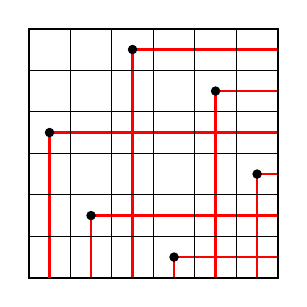
\begin{tikzpicture}[x=1.5em,y=1.5em]
      \draw[color=black, thick](0,1)rectangle(6,7);
      \draw[color=black](1,4)rectangle(2,5);
      \draw[color=black](3,4)rectangle(4,5);
       \draw[color=black](1,3)rectangle(2,4);
      \draw[color=black](3,3)rectangle(4,4);
      \draw[color=black](1,2)rectangle(2,3);
      \draw[color=black](0,1)rectangle(1,2);  
     \draw[thick,color=red] (6,6.5)--(2.5,6.5)--(2.5,1);      
     \draw[thick,color=red] (6,5.5)--(4.5,5.5)--(4.5,1);
     \draw[thick,color=red] (6,4.5)--(0.5,4.5)--(0.5,1);
     \draw[thick,color=red] (6,3.5)--(5.5,3.5)--(5.5,1);
     \draw[thick,color=red] (6,2.5)--(1.5,2.5)--(1.5,1);
     \draw[thick,color=red] (6,1.5)--(3.5,1.5)--(3.5,1);
     \filldraw [black](0.5,4.5)circle(.1);
      \filldraw [black](5.5,3.5)circle(.1);
     \filldraw [black](4.5,5.5)circle(.1);
     \filldraw [black](3.5,1.5)circle(.1);
      \filldraw [black](1.5,2.5)circle(.1);
      \filldraw [black](2.5,6.5)circle(.1);
      \draw[color=black](0,6)rectangle(1,7);
      \draw[color=black](1,6)rectangle(2,7);  
      \draw[color=black](2,6)rectangle(3,7);
      \draw[color=black](3,6)rectangle(4,7); 
      \draw[color=black](4,6)rectangle(5,7);
      \draw[color=black](5,6)rectangle(6,7);
      \draw[color=black](0,5)rectangle(1,6);
      \draw[color=black](1,5)rectangle(2,6);  
      \draw[color=black](2,5)rectangle(3,6);
      \draw[color=black](3,5)rectangle(4,6); 
      \draw[color=black](4,5)rectangle(5,6);
      \draw[color=black](5,5)rectangle(6,6);
     \draw[color=black](0,4)rectangle(1,5); 
      \draw[color=black](2,4)rectangle(3,5);
      \draw[color=black](4,4)rectangle(5,5);
      \draw[color=black](5,4)rectangle(6,5);
      \draw[color=black](0,3)rectangle(1,4); 
      \draw[color=black](2,3)rectangle(3,4);
      \draw[color=black](4,3)rectangle(5,4);
      \draw[color=black](5,3)rectangle(6,4);
      \draw[color=black](0,2)rectangle(1,3); 
      \draw[color=black](2,2)rectangle(3,3);
      \draw[color=black](3,2)rectangle(4,3);
      \draw[color=black](4,2)rectangle(5,3);
      \draw[color=black](5,2)rectangle(6,3);
      \draw[color=black](1,1)rectangle(2,2);  
      \draw[color=black](2,1)rectangle(3,2);
      \draw[color=black](3,1)rectangle(4,2); 
      \draw[color=black](4,1)rectangle(5,2);
      \draw[color=black](5,1)rectangle(6,2);
     \end{tikzpicture}.
\] 
Then \[
I_w = (z_{1,1}, z_{1,2}, z_{2,1}, z_{2,2}, 2\text{-minors in } (Z_w)_{[4],[2]},  2\text{-minors in } (Z_w)_{[2],[4]}, 3\text{-minors in } (Z_w)_{[4],[4]})
\] and  \[
Q_{y,I_w} = (2\text{-minors in } (Z_w)_{[4],[2]},  2\text{-minors in } (Z_w)_{[2],[4]}, 2\text{-minors in } (Z_w)_{[3],[3]}).
\] The $2$-minors in $(Z_w)_{[2],[4]}$, for example, are included as generators of $Q_{y,I_w}$ because \[
\rank_w(4,4)+1 = 3<4 = \min\{4,4\} = \min\{m_1,m_2\}
\] and $(2,4) \in \Ess(w)$ is in the same column as $(4,4)$.  
\end{example}

We make this definition purely for technical convenience below and not out of an independent interest in $\Spec(R/Q_{y,I_w})$.  We will say that $Q_{y,I_w}$ is CDG if the generators given above form a Gr\"obner basis under any diagonal term order.  
